\section{Evaluation}
\label{sec:eval}

\iffalse
Evaluation (don't forget to interpret your data)
\fi

\subsection{Experiment platform}

The experiment platform is shown in the table.

\begin{table}[ht]

\begin{tabular}{|l|l|}
\hline 
Name & Version \\ 
\hline 
CPU & 4 cores, Intel(R) Core(TM) i7-3770 \\
& CPU @ 3.4GHz \\ 
\hline 
Memory & 16 GB \\ 
\hline 
Operating System & Ubuntu 14.04.2 LTS \\ 
\hline 
Hadoop & Version 2.6.0, per \\ 
\hline 
Docker & Version 1.5.0, build a8a31ef \\ 
\hline 
Disk & Usage less than 90\% \\ 
\hline 
\end{tabular}
\end{table}


\subsection{Hadoop setup with Docker configuration}

We suppose that Hadoop is already installed in Pseudo-Distributed mode, and Docker is also installed. Firstly, we download docker image for Hadoop docker container.Then, we add the following properties to yarn-site.xml:

\begin{figure}[h]
  \centering
  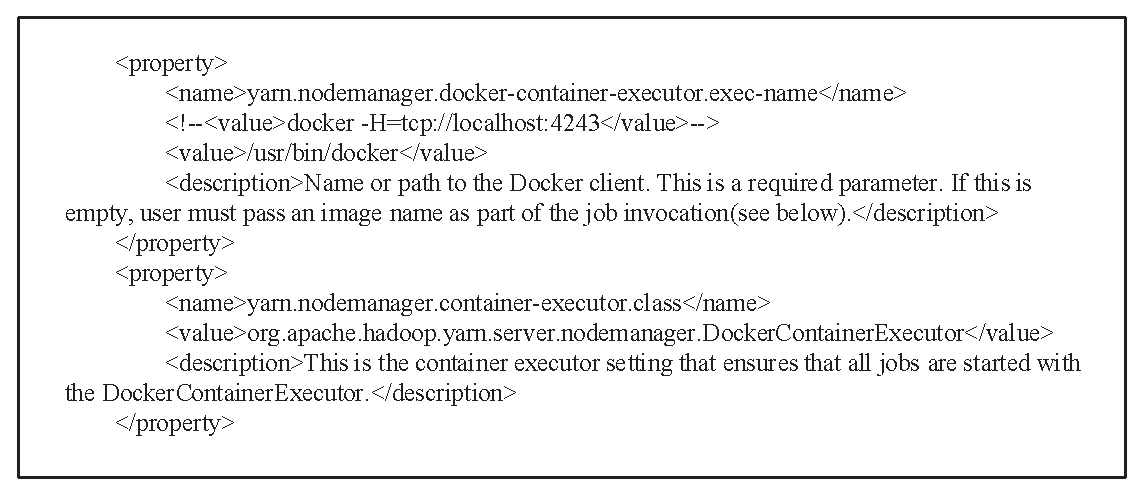
\includegraphics[width=3in]{figs/code.eps}
  \label{fig:Codeoverview}
\end{figure}

In order for Hadoop to use Docker container, we need to change the permission of docker command with “sudo chmod u+s /usr/bin/docker”.

Go to the directory of Hadoop installation, and start Hadoop with “sbin/start-dfs.sh” and “sbin/start-yarn.sh”. 

The results of  “jps” command will present you the running processes: NameNode, SecondaryNameNode, DataNode, ResourceManager, NodeManager.

To test the usage of Docker container in Hadoop, we use one Hadoop example program teragen to generate 1000 bytes of data. The command is as follows:

\begin{figure}[h]
  \centering
  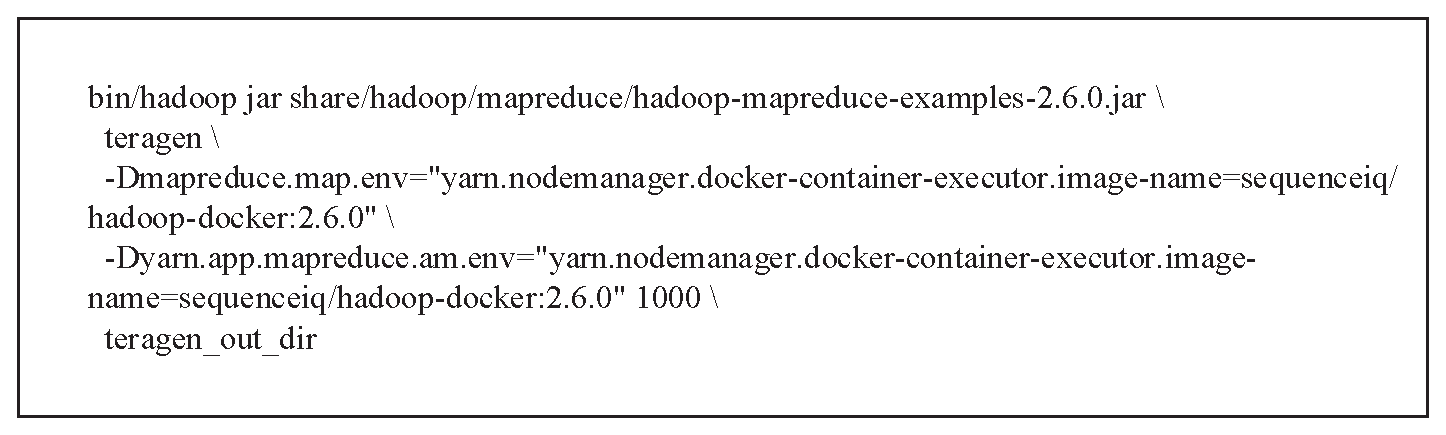
\includegraphics[width=3in]{figs/command.eps}
  \label{fig:Commandoverview}
\end{figure}

After the job is launched to execute, “docker ps” command shows that there are 3 containers that are launched to run the Teragen program. The 3 containers terminate after the job is finished.

\subsection{Example attack}

Since docker is being able to run by any user, use “docker stop containerID” could terminate the containers which are running MapReduce jobs. In this way, the malicious user could introduce failures to jobs. The screenshot is shown as below.

\begin{figure}[t]
  \centering
  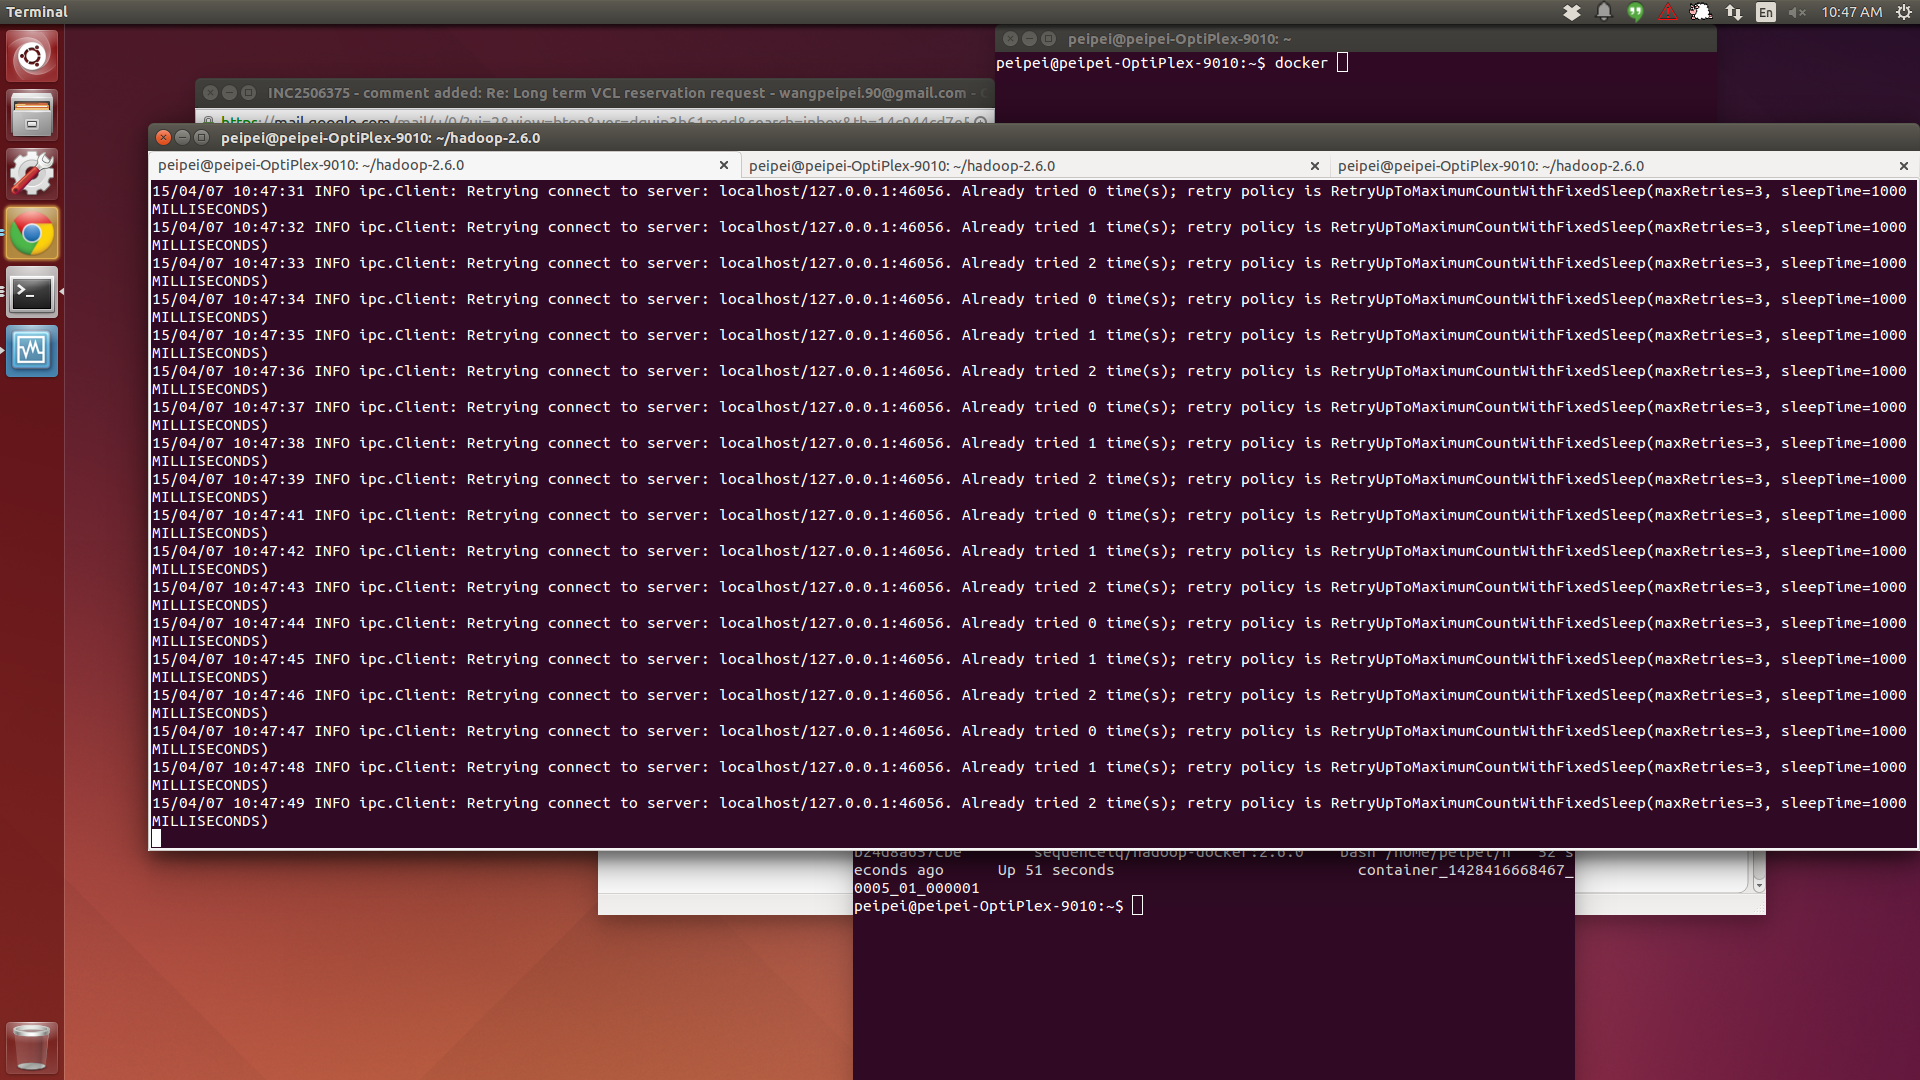
\includegraphics[width=3in]{figs/attack.png}
  \caption{Attack experiment}
  \label{fig:attackoverview}
\end{figure}